\subparagraph{Задание 4.7}

\textbf{Условие}:
Вывести в окне Watch (View->Watch) содержимое выходного буфера. 

\textbf{Решение}:

Жмем \textbf{F10}. Жмем два раза \textbf{влево}. \textbf{Enter}. Жмем три раза \textbf{вниз}. \textbf{Enter}.
Рисунок~\ref{fig:task_4_7__menu_watches} (стр.~\pageref{fig:task_4_7__menu_watches}).

Вводим watch, например, 21h. Нажимаем ОК (\textbf{Enter}).
Рисунок~\ref{fig:task_4_7__watches_21h} (стр.~\pageref{fig:task_4_7__watches_21h}).

Результат на рисунке~\ref{fig:task_4_7__watches_result} (стр.~\pageref{fig:task_4_7__watches_result}).

\begin{figure}[!htp]
    \centering
    \begin{minipage}{0.32\textwidth}
        \centering
        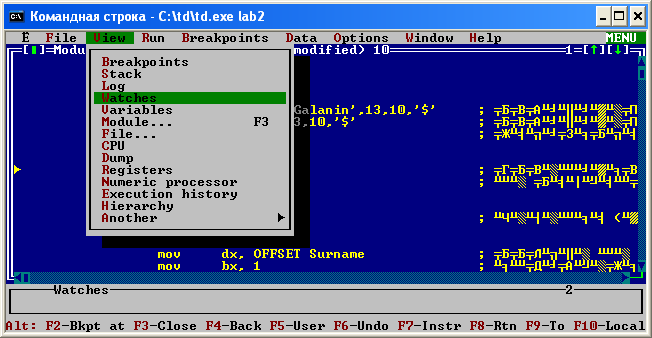
\includegraphics[width=.99\linewidth]
            {../_INCLUDES/task-4-7/td-view-watches.png}
        \caption{>\textbf{View}>\textbf{Wathes}}
        \label{fig:task_4_7__menu_watches}
    \end{minipage}
    \begin {minipage}{0.32\textwidth}
        \centering
        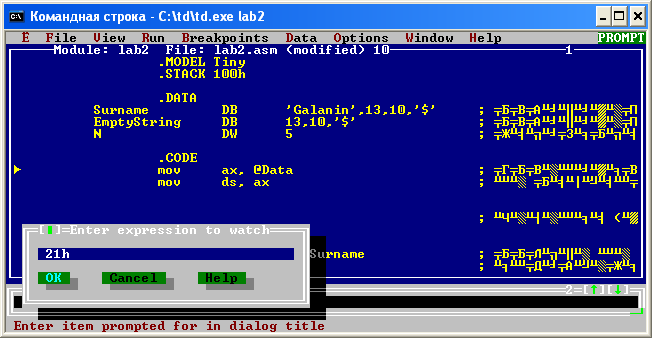
\includegraphics[width=.99\linewidth]
            {../_INCLUDES/task-4-7/watch-21h.png}
        \caption{Пишем watch}
        \label{fig:task_4_7__watches_21h}
    \end{minipage}
    \begin {minipage}{0.32\textwidth}
        \centering
        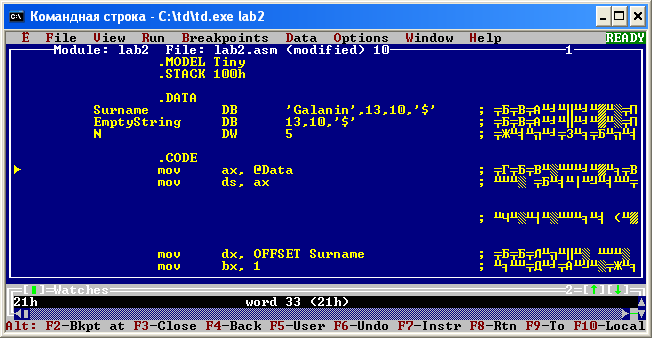
\includegraphics[width=.99\linewidth]
            {../_INCLUDES/task-4-7/watch-result.png}
        \caption{Результат watch}
        \label{fig:task_4_7__watches_result}
    \end{minipage}
\end{figure}
